\section*{Results and Discussion}
\subsection*{Determination of system structural details}
In order to construct an initial configuration which gives reliable 
trends, we need to understand the composition of layers, how far apart
to stack the layers, and how to orient them with respect to each other.
To verify our choices for each parameter, we compare our calculations
to experimental small angle X-ray scattering (SAXS), wide angle X-ray
scattering (WAXS), and ionic conductivity measurements.

To discern the composition of the monomer layers, we ran simulations of 
systems created with 4 - 8 monomers per layer. Both the sandwiched and 
parallel displaced configurations were tested. All systems remained
stable for at least 50 ns. Pore spacings were calculated by measuring
the distance between the pore centers. Pore centers were located by
averaging the coordinates of sodium ions in their respective pores. 
Statistics were generated using the bootstrapping technique. Table
~\ref{table:p2p} shows the pore spacing for all systems tested.
Systems built with 5 monomers in each layer equilibrate to a pore
spacing that is most consistent with the experimental value of 4.12 nm
derived from SAXS measurements (Figure~\ref{fig:SAXS}). The remainder of
this discussion will focus on the analysis of systems built with 5 
monomers per layer. Pair correlation functions calculated between 
aromatic rings along the length of the pores indicate that systems
prefer to stay partitioned into layers (Fig~\ref{fig:zdf}).

\begin{table}
\centering
\begin{tabular}{|c|c|c|}
\toprule
                   & \multicolumn{2}{c}{Starting Configuration} \\
Monomers per layer & Sandwiched & Parallel Displaced \\
\midrule
4 & $3.71 \pm 0.08$ & $3.82 \pm 0.06$ \\
5 & $3.99 \pm 0.08$ & $4.16 \pm 0.09$ \\
6 & $4.83 \pm 0.08$ & $4.85 \pm 0.05$ \\
7 & $4.73 \pm 0.06$ & $4.84 \pm 0.06$ \\
8 & $5.08 \pm 0.08$ & $5.46 \pm 0.07$ \\
\bottomrule
\end{tabular}
\caption{The pore spacing of the model increases as number of monomers
in each layer increases. The pore spacing of a system starting in the 
sandwiched configuration is systematically lower than that started in an 
offset configuration. Systems built with 5 monomers per layer in a parallel
displaced configuration results in a pore spacing closest to experimental
data}\label{table:p2p} 
\end{table}

\begin{figure}
	\centering
	\begin{subfigure}{0.45\textwidth}
		\centering
		\includegraphics[width=\textwidth]{zdf5layered.png}
		\caption{}\label{fig:zdf_layered}
	\end{subfigure}
	\begin{subfigure}{0.45\textwidth}
		\centering
		\includegraphics[width=\textwidth]{zdf5offset.png}
		\caption{}\label{fig:zdf_offset}
	\end{subfigure}
	\caption{Pair distribution functions of aromatic carbons for the
	(a) 5 monomer per layer, sanwiched and (b) 5 monomer per layer, 
	parallel displaced configurations. Spikes in the distribution mark
	distinct layers. The magnitude of the spikes with respect to the 
	average suggest that the 5 monomer per layer, sandwiched configuration
	possesses the highest degree of layer partitioning.}\label{fig:zdf}
\end{figure}

The experimental 2D WAXS measurement contains five major reflections which
our model intends to reproduce (Figure~\ref{fig:WAXS}). The first is located
at qz = 1.7 \angstrom \textsuperscript{-1}, corresponding to a real space 
spacing of 3.7 \angstrom. The reflection is attributed to pi-pi stacking
between aromatic rings in the direction perpendicular to the membrane plane, or z-axis. 
For simplicity, this reflection will be referred to as R-pi. A weak intensity
line is located at exactly half the qz value of R-pi (qz = 0.85 \angstrom \textsuperscript{-1}), corresponding to a 
real space periodic spacing of 7.4 \angstrom. This reflection has been 
interpreted  as 2\textsubscript{1} helical ordering of aromatic rings along the
z axis and will therefore be referred to as R-helix. If positions of the 
aromatic rings can be traced by a helix, then for each turn in the helix, 
there should be two aromatic rings. A third major reflection is marked by 
a low intensity ring located at r = 1.4 \angstrom \textsuperscript{-1}. The
real space separation corresponds to 4.5 \angstrom which is characteristic
of the average spacing between packed alkane chains. This reflection will be
called R-alkanes. Within R-alkanes, are four spots of higher intensity which 
will be called R-spots. All are located $\approx 40$ degrees from the qz axis
in their respective quadrants. In many liquid crystal systems this can be
explained by the tilt angle of the alkane chains with respect to the xy plane. 
The final major reflections correspond to the spacing and symmetry of the d100 
plane which can be related to the distance between pores. The feature, which 
will be called R-pores, is characterized by dots along qz = 0. The spacing
between dots is indicative of the hexagonal symmetry of the packed pores. It
is easiest to interpret the data by radially integrating the 2D data to get 
a 1D curve which is shown in Figure~\ref{fig:SAXS}.

\begin{figure}
	\centering
	\begin{subfigure}[t]{0.47\linewidth}
		\centering
		\raisebox{.2\textwidth}{%
		\includegraphics[width=\linewidth]{WAXS_soft_confined.png}
		}
		\caption{}\label{fig:WAXS}
	\end{subfigure}
	\begin{subfigure}[t]{0.43\linewidth}
		\centering
	%	\vspace{12mm}
		\includegraphics[width=\linewidth]{SAXS.png}
		\caption{}\label{fig:SAXS}
	\end{subfigure}
	\caption{(a) 2D wide angle X-ray scattering gives details about repeating features less than 1 nanometer apart. (b) 1D small angle X-ray scattering indicates hexagonal packing of pores as well as the spacing between pores.}\label{fig:SWAXS}
\end{figure}

The initial distance between layers can influence the approach towards
equilibrium. Equilibrated systems built according to the 3.7 \angstrom 
spacing indicated by R-pi are characterized by a defined, cylindrical and
open pore structure. Aromatic rings are arranged in a helical conformation.
We will refer to this system as Basin A (Figure~\ref{fig:280K_pore}). Simulations
of systems built with layers stacked greater than 4 \angstrom apart results in a pore
structure characterized by high radial disorder, while still maintaining 
partitioning between hydrophobic and hydrophilic regions. This will be 
called Basin B (Figure~\ref{fig:340K_pore}). It is apparent that this LLC membrane
may exist in at least two metastable states. The distinct difference in 
pore structure exhibited by each phase will likely lead to different transport
mechanisms. Understanding which phase exists experimentally is necessary in 
order to appropriately study the system.
% BJC: include more examples of the difference between the two basins
% The arrangement of sodium ions (which are closely bound to carbonyl
% head groups) can be well-approximated by a gaussian distribution 
% Like phase A, phase B can form at 280K. 
% The phase is also present when phase A is heated close to its isotropic transition point
% There are distinct differences in the membrane and pore structures between each state (Fig~\ref{fig:porestructures})

Basin A and Basin B are two configurationally metastable basins. 
We hesitate to classify the basins as separate phases. We hypothesize
that Basin B is present at higher temperatures. This is evidenced by
a simulation of a system in Basin A whose temperature was linearly
ramped from 280K to 340K over 100 ns. Visually, there is a distinct
change in pore structure from one characteristic of Basin A 
(Figure~\ref{fig:280K_pore}) to one characteristic of Basin B 
(Figure~\ref{fig:340K_pore}). To quantify our observation, we chose 
three easily measurable order parameters: the distance between pores,
the membrane the thickness and the ratio of pore radius to the uncertainty
in pore radius. The distance between pores was measured as described 
previously. The membrane thickness was measured using the length of the
z box vector. The pore radius was measured by calculating the distance
between the center of mass of each aromatic ring and the center of mass
of all aromatic rings in respective pores. The pore radius is divided by
its uncertainty in order to understand the degree to which monomers 
obstruct the pore region. Referring back to our temperature ramped system,
the slope of all order parameters change around 315K - 325K 
(\Cref{fig:p2p_tramp,fig:thickness_tramp,fig:order_tramp}) indicating the 
possibility of an abrupt change in system ordering. To prove that the 
basins are in fact two different phases, we must observe evidence of a
first order phase transition, which would be indicated by a discontinuity
in an order parameter as a function of temperature. Our 100 ns temperature
ramp may have been too fast causing the system to suffer from hysteresis. To mitigate
hysteresis, we performed a slow, stepwise temperature ramp. Starting from
structures equilibrated at 280K, the system temperature was raised to 
300K and allowed to equilibrate for 200 ns. At the end of 200 ns, the
temperature was raised 5K and equilibrated again for 200 ns. We repeated
this process until the system was equilibrated for 200 ns at 320K. In all
cases, we observed smooth changes in order parameters as temperature was
increased implying that we can not yet claim the existence of two phases (Figure~\ref{fig:phase_transition}).
The same process will continue to be repeated up to 340K in the near future
since we have not surpassed the temperatures where we observe abrupt slope 
changes in pore spacing and membrane thickness (\Cref{fig:p2p_tramp,fig:thickness_tramp}).

\begin{figure}
        \centering
        \begin{subfigure}[b]{0.45\textwidth}
                \centering
                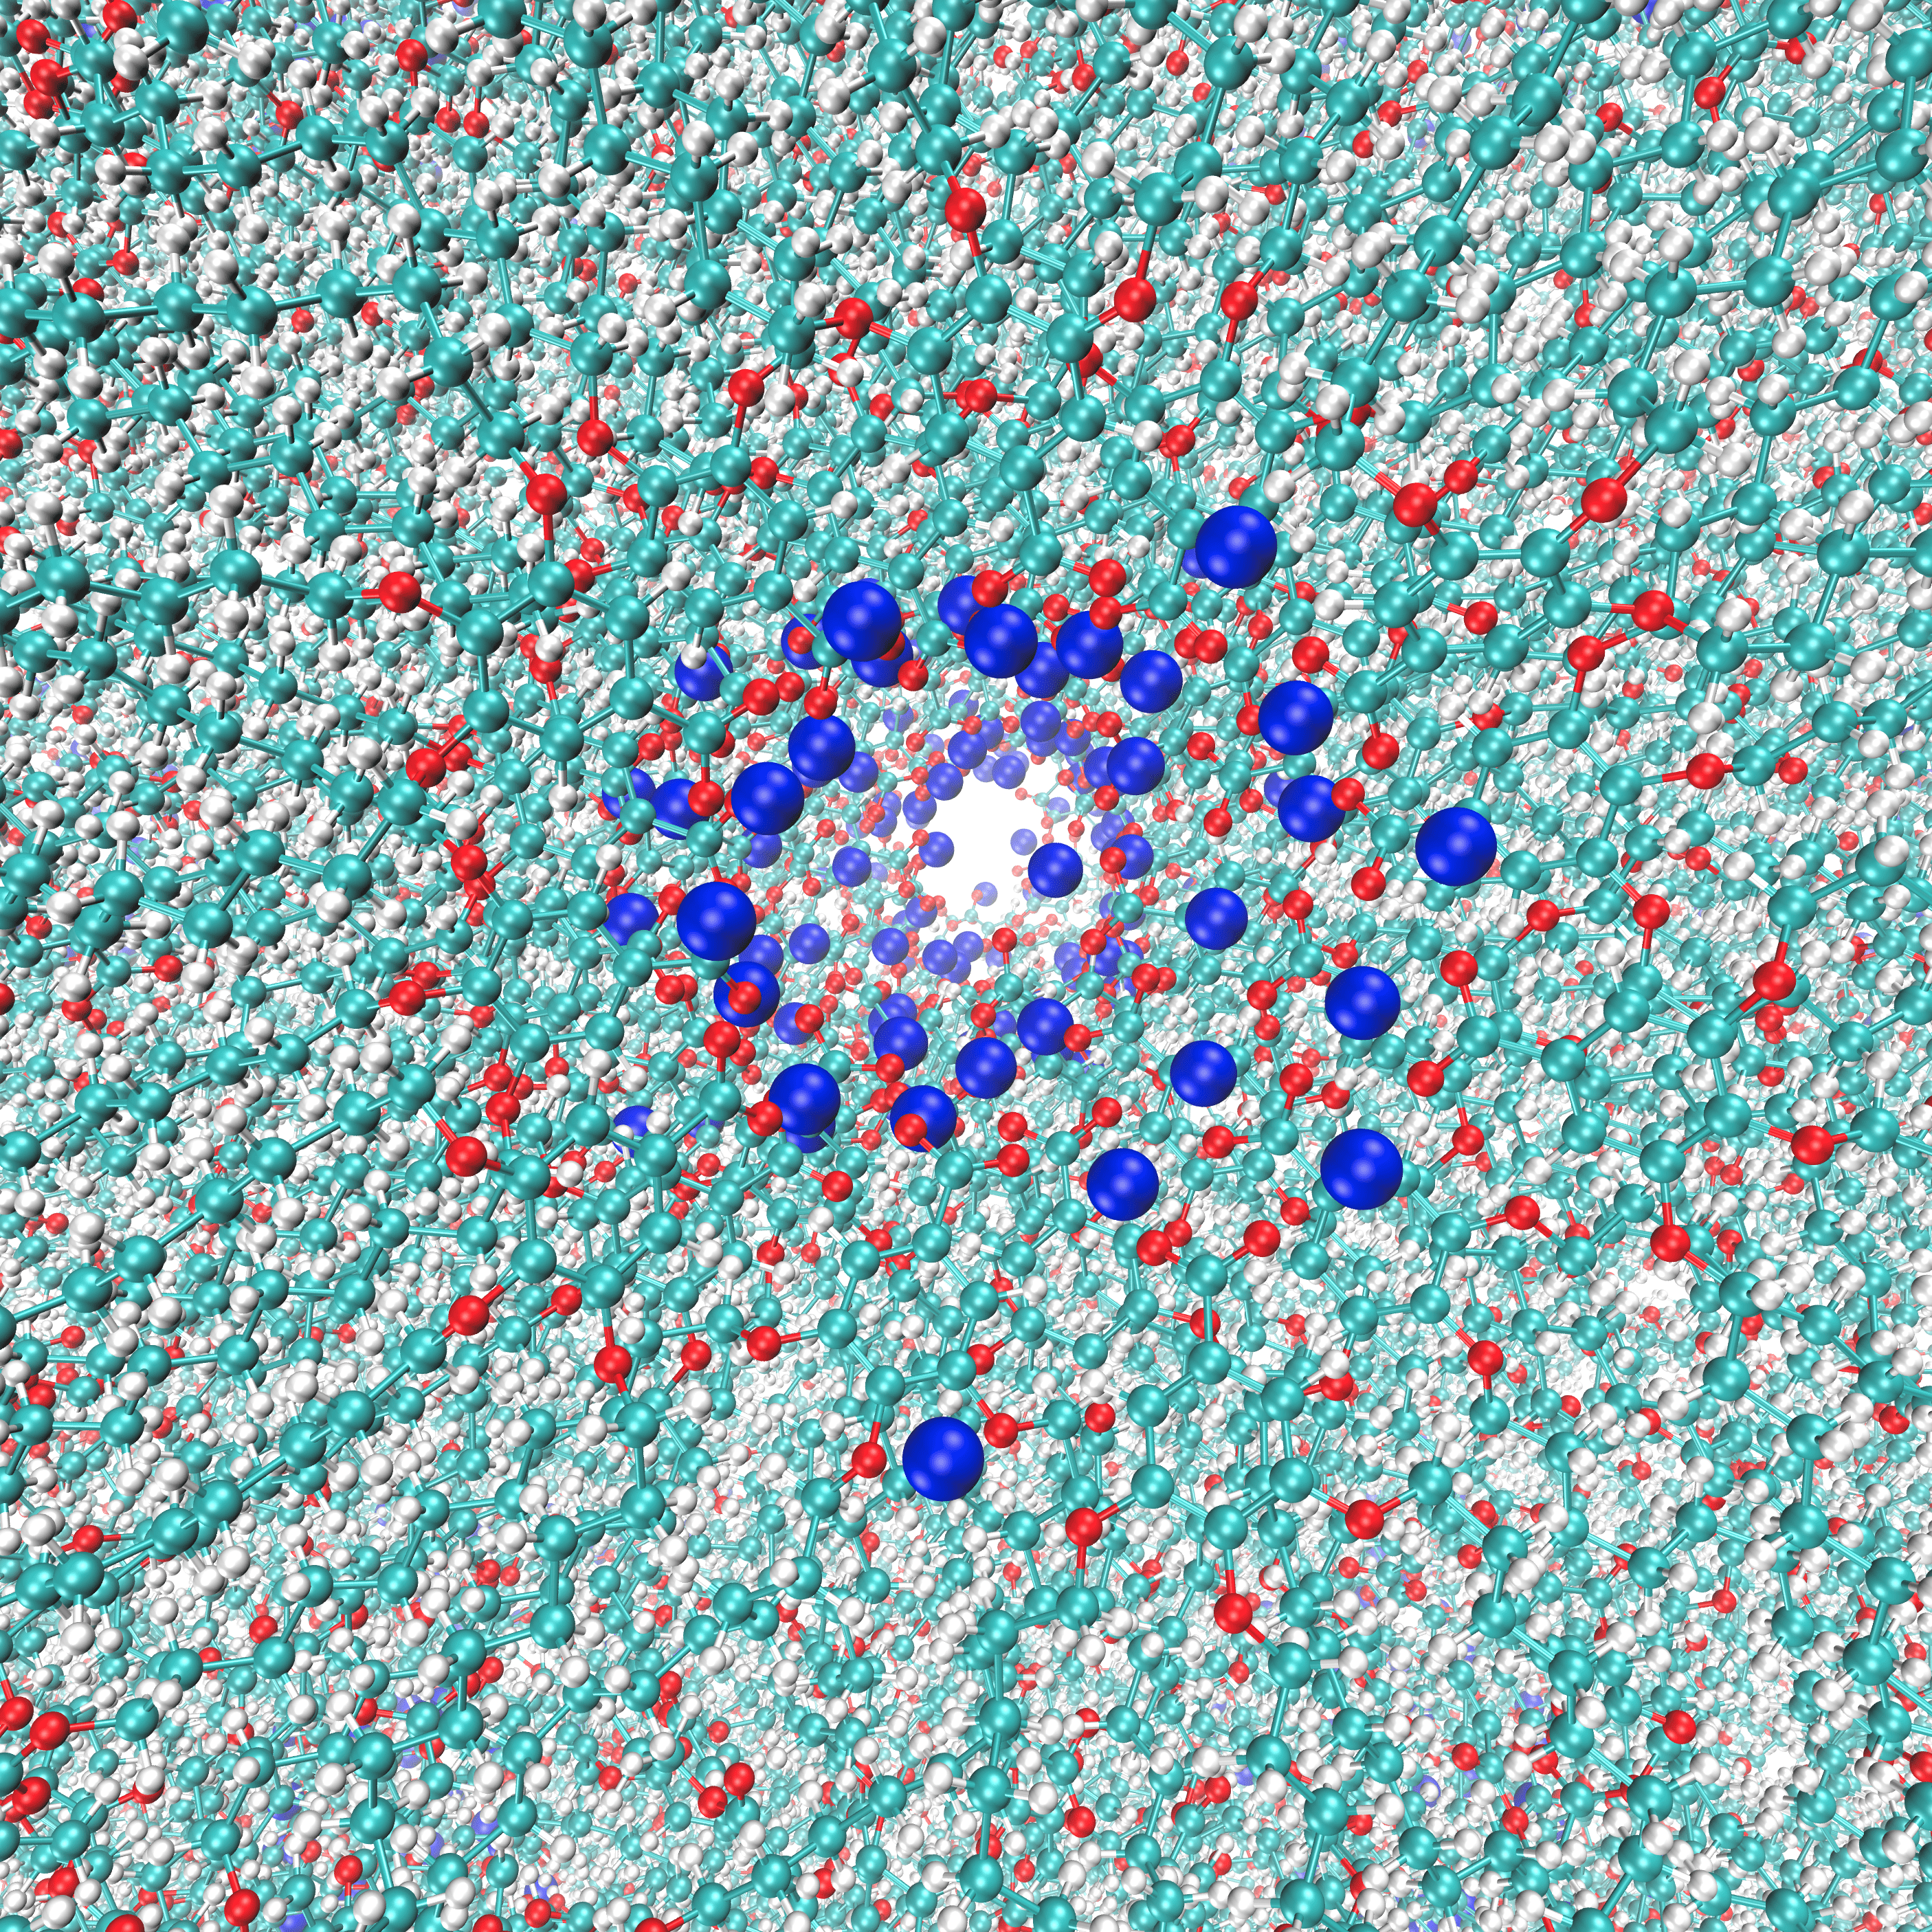
\includegraphics[width=\textwidth]{280K_tramp_close.png}
                \caption{}\label{fig:280K_pore}
        \end{subfigure}
        \begin{subfigure}[b]{0.45\textwidth}
                \centering
                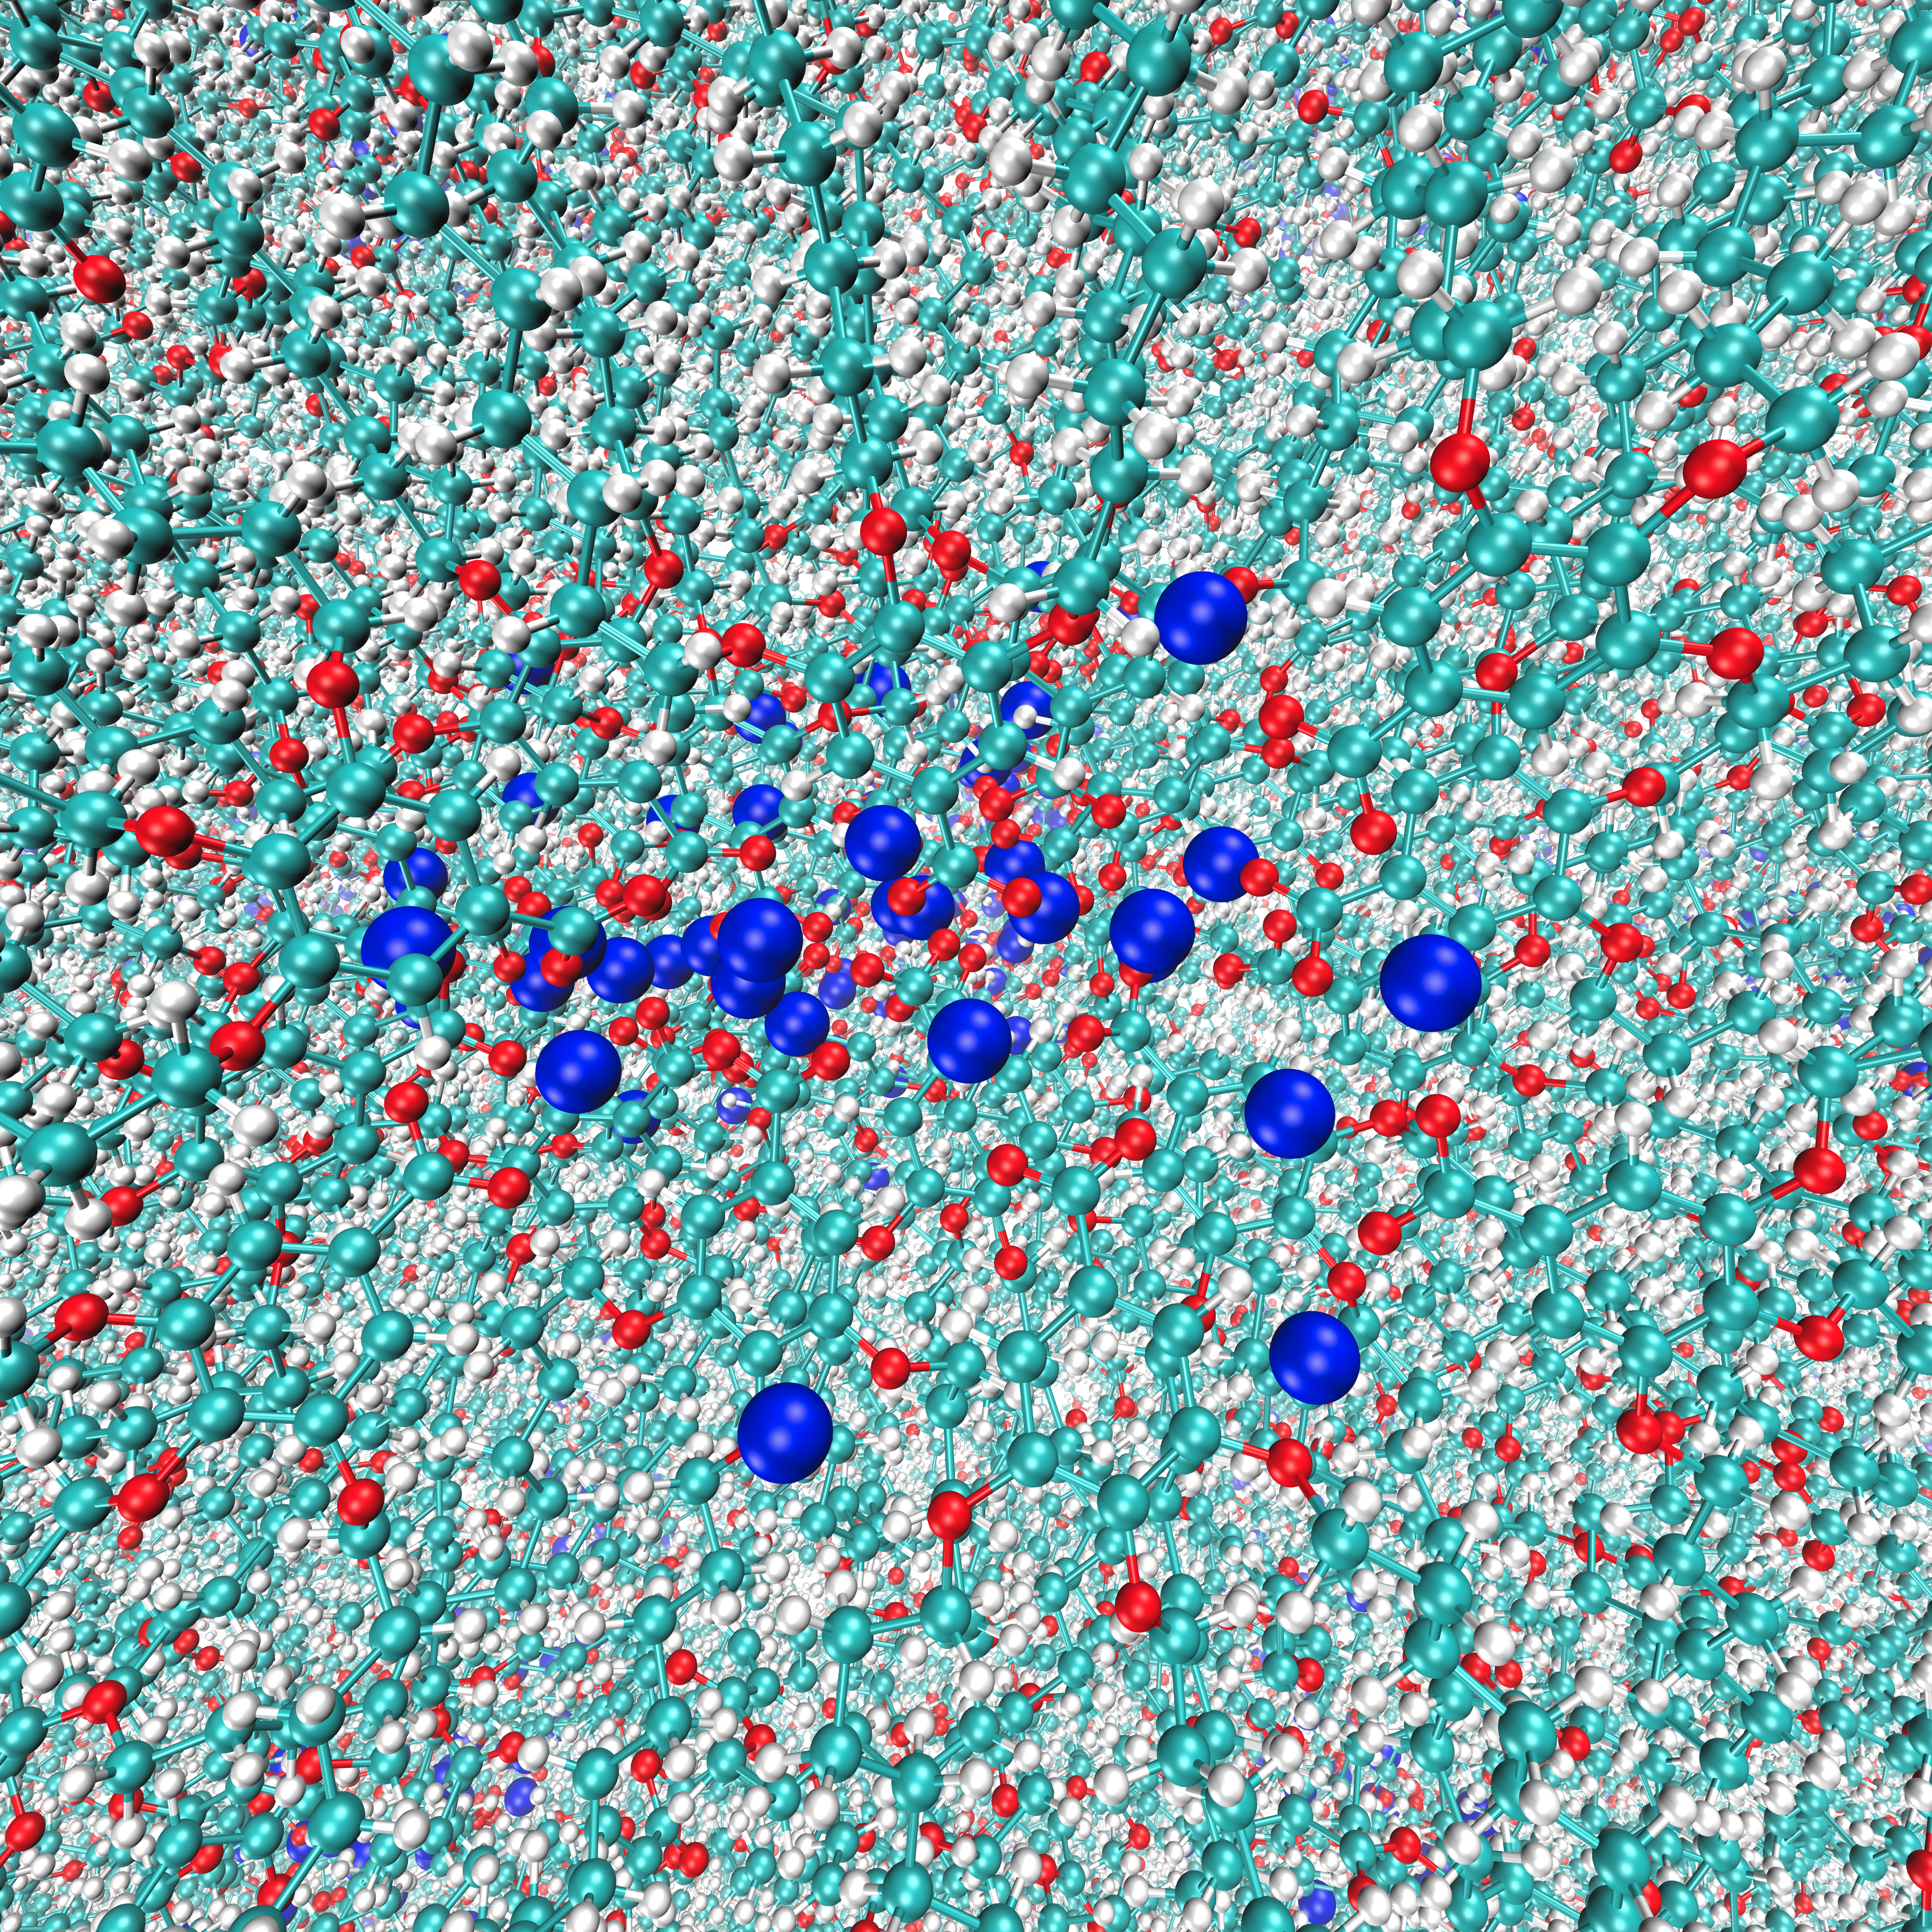
\includegraphics[width=\textwidth]{340K_tramp_close.png}
                \caption{}\label{fig:340K_pore}
        \end{subfigure}
        \vskip\baselineskip
        \begin{subfigure}[b]{0.325\textwidth}
                \centering
                \includegraphics[width=\textwidth]{p2p_tramp.png}
                \caption{}\label{fig:p2p_tramp}
        \end{subfigure}
        \begin{subfigure}[b]{0.325\textwidth}
                \centering
                \includegraphics[width=\textwidth]{thickness_tramp.png}

                \caption{}\label{fig:thickness_tramp}
        \end{subfigure}
        \begin{subfigure}[b]{0.325\textwidth}
                \centering
                \includegraphics[width=\textwidth]{order_tramp.png}
                \caption{}\label{fig:order_tramp}
        \end{subfigure}
        \caption{(a) The open pore structure exhibited by a structure equilibrated
	at 280K is characteristic of Basin A. (b) The closed pore structure with 
	a high degree of radial disorder exhibited when the structure in (a) is 
	heated to 340K is characteristic of Basin B. (c) A plot of distance between pores
	vs. temperature changes slope near 325K. (d) A plot of membrane thickness vs. 
	temperature changes slope near 325K. (e) The plot of the ratio of pore radius to
	its uncertainty changes slope near 315K.}\label{fig:tramp}
\end{figure}

\begin{figure}
	\centering
	\begin{subfigure}{0.325\textwidth}
		\centering
		\includegraphics[width=\textwidth]{p2p_layered.png}
		\caption{}\label{fig:p2p_layered}
	\end{subfigure}
	\begin{subfigure}{0.325\textwidth}
		\centering
		\includegraphics[width=\textwidth]{thickness_layered.png}
		\caption{}\label{fig:thickness_layered}
	\end{subfigure}
	\begin{subfigure}{0.325\textwidth}
		\centering
		\includegraphics[width=\textwidth]{order_layered.png}
		\caption{}\label{fig:order_layered}
	\end{subfigure}
	\caption{In all cases, blue lines represent the measured value of
	the order parameter, black lines are average values calculated from
	equilibrated Basin B systems at each temperature, green shaded regions
	represent the standard deviation of each of the black line values, and 
	red dashed lines show where the temperature is bumped to the next level.
	(a) The pore spacing decreases smoothly as it approaches Basin B values.
	(b) Membrane thickness increases steadily with temperature, however
	it is still far from the Basin B value after 200 ns at 320K. (c) The
	ratio of pore radius to is uncertainty rapidly decreases initially and
	approaches the Basin B value smoothly until they finally overlap at 320K.}\label{fig:phase_transition}
\end{figure}

We varied the relative interlayer orientation between sandwiched and 
parallel-displaced based on our knowledge of the stability of these two
pi-stacking modes. Short NVT simulations were run with position restraints
on aromatic ring carbon atoms. Simulated X-ray diffraction patterns 
generated from each configuration establish a difference between the two
stacking modes (Figure~\ref{fig:XRDrestrained}). In each pattern, R-alkanes is present at a distance of
$\approx 1.5$ \angstrom \textsuperscript{-1}. R-pi is also present in each 
pattern, although it appears to intersect R-alkanes because the spacing
between aromatic rings is similar to the alkane chain packing. The difference 
in aromatic ring spacing between experiment and simulation is likely a result
of the inability of GAFF to properly handle aromatic interactions. The parallel
displaced configuration contains two lines of high intensity with maximum
intensity occurring where they intersect the alkane chain region due to
constructive interference between the two features. The lines are located
where one would expect to see R-helix. As the simulation is progressed, 
the full line begins to fade and the reflection persists only at the 
intersection with the R-alkanes. Most significantly, the line is no
longer present where R-helix exists and, perhaps coincidentally, the 
intersection with R-alkanes occurs where one would expect to see R-spots.

\begin{figure}
	\centering
	\begin{subfigure}{0.475\textwidth}
		\centering
		\includegraphics[width=\textwidth]{rzlayeredrestrained.png}
		\caption{}\label{fig:rzplayeredrestrained}
	\end{subfigure}
	\begin{subfigure}{0.475\textwidth}
		\centering
		\includegraphics[width=\textwidth]{rzoffsetrestrained.png}
		\caption{}\label{fig:rzoffsetrestrained}
	\end{subfigure}
	\caption{(a) Simulated X-ray diffraction of a sandwiched configuration
	with restraints placed on aromatic carbons shows all major features
	present experimental WAXS. Near solid lines at constant z are a result of 
	the highly ordered aromatic rings. (b) Simulated X-ray diffraction of a similarly
	restrained parallel displaced configuration may also contained all
	major experimental WAXS features. One can argue that R-spots is not present
	but it is difficult to distinguish because of its intersection with the solid
	R-helix line. Longer simulations are necessary to determine which structure
	is the best match to experiment}\label{fig:XRDrestrained}
\end{figure}

Full comparison of experimental 2D WAXS with simulated X-ray diffraction
patterns produced from equilibrated MD trajectories shows the most consistency
with the sandwiched conformation in Basin A. Systems were built in both the 
parallel displaced and sandwiched conformations with an intial layer spacing of
3.7 \angstrom. A third system was created by stacking layers in the sandwiched 
conformation 5 \angstrom apart in order to guide it towards Basin B. For ease of
reference, the third system will be referred to as the disordered system. The 
three systems were equilibrated according to our procedure with NPT simulations of 
greater than 400 ns. Simulated diffration patterns were generated using 
portions of the trajectory after equilibration (Figure~\ref{fig:XRDsim}). Equilibration was detected
when the distance between pores and the membrane thickness stopped changing.
Simulated diffraction patterns for all three structures are shown in 
Fig~\ref{fig:XRDsim}. The equilibrated parallel displaced structure exhibits 
R-alkanes and R-pores in the expected locations. Due to low resolution, making
out the individual spots of R-pores is challenging and can be validated upon
further inspection of the 3D structure factor. R-pi is also present, however it
intersects R-alkanes because it is at a lower q than expected. This can be 
explained by our model's inability to appropriately represent aromatic interactions.
The rings prefer to stack $\approx 4.1 \angstrom$ apart as opposed to 3.7 \angstrom.
R-helix and R-spots are both missing. The line which intersected both of these
features in the restrained simulations faded upon equilibration which suggests
that monomers in the parallel-displaced conformation may not give rise to the 
experimental WAXS pattern seen. Simulated XRD of the sandwiched configuration 
contains all features except for R-helix. Most notably, R-spots appears in the
expected location, which suggests that there is something intrinsic to
the sandwiched packing which gives rise to such features. Finally, the 
disordered structure exhibits R-alkanes and R-pores. R-helix and R-spots are not
present. Given the evidence, the sandwiched configuration with layers spaced
3.7 \angstrom apart gives rise to an equilibrated structure closest to experiment. 

\begin{figure}
	\centering
	\begin{subfigure}{0.31\textwidth}
		\centering
		\includegraphics[width=\textwidth]{sandwich_rzplot.png}
		\caption{}\label{fig:sandwich_rzplot}
	\end{subfigure}
	\begin{subfigure}{0.31\textwidth}
		\centering
		\includegraphics[width=\textwidth]{offset_rzplot.png}
		\caption{}\label{fig:offsetrzplot}
	\end{subfigure}
	\begin{subfigure}{0.31\textwidth}
		\centering
		\includegraphics[width=\textwidth]{disorder_rzplot.png}
		\caption{}\label{fig:disorder_rzplot.png}
	\end{subfigure}
	\caption{(a) All major features except R-helix are present in
	XRD patterns resulting from an equilibrated sandwiched configuration 
	in Basin A. R-pi intersescts R-alkanes. R-helix faded during equilbration.
	(b) All major features execpt R-spots are present in XRD patterns 
	resulting from an equilibrated parallel displaced configuration in Basin A.
	R-helix exists faintly in the expected location. (c) R-pores and R-alkanes
	are the only major features present in XRD patterns resulting from an 
	equilibrated disordered phase}\label{fig:XRDsim}
\end{figure}

The spots that appear in the simulated XRD pattern of the sandwiched
conformation are a result of the way alkane tails pack together. Previously,
the spots in the diffraction pattern had been explained as the product of
tilted alkane chains. We measured the tilt angle of the alkane chains and 
showed that our system equilibrates to an average tilt angle close to zero 
degrees (Fig~\ref{fig:tilt}). To understand the origin of the spots, we 
determined which atoms gave rise to the feature. By removing atoms from 
the trajectory and simulating a diffraction pattern, we were able to isolate
the cause of the spots to the tails. Since the tails are mostly flat, we
plotted the centroids of the tails and measured the angle between each centroid 
and its nearest neighbors with respect to the plane of the membrane. The 
distribution of these angles is consistent with the location of the spots.
We reason that monomer tails stacked closely in the sandwiched conformation
are forced to splay apart and pack in between in each other which creates a
nearly hexagonal array of packed tails. 

\begin{wrapfigure}{R}{0.4\textwidth}
	\centering
	\includegraphics[width=0.4\textwidth]{tilt.png}
	\caption{The average angle between alkyl chains and the xy plane is nearly zero degrees}\label{fig:tilt}
\end{wrapfigure}

\begin{figure}
	\centering
	\begin{subfigure}{0.45\textwidth}
		\centering
		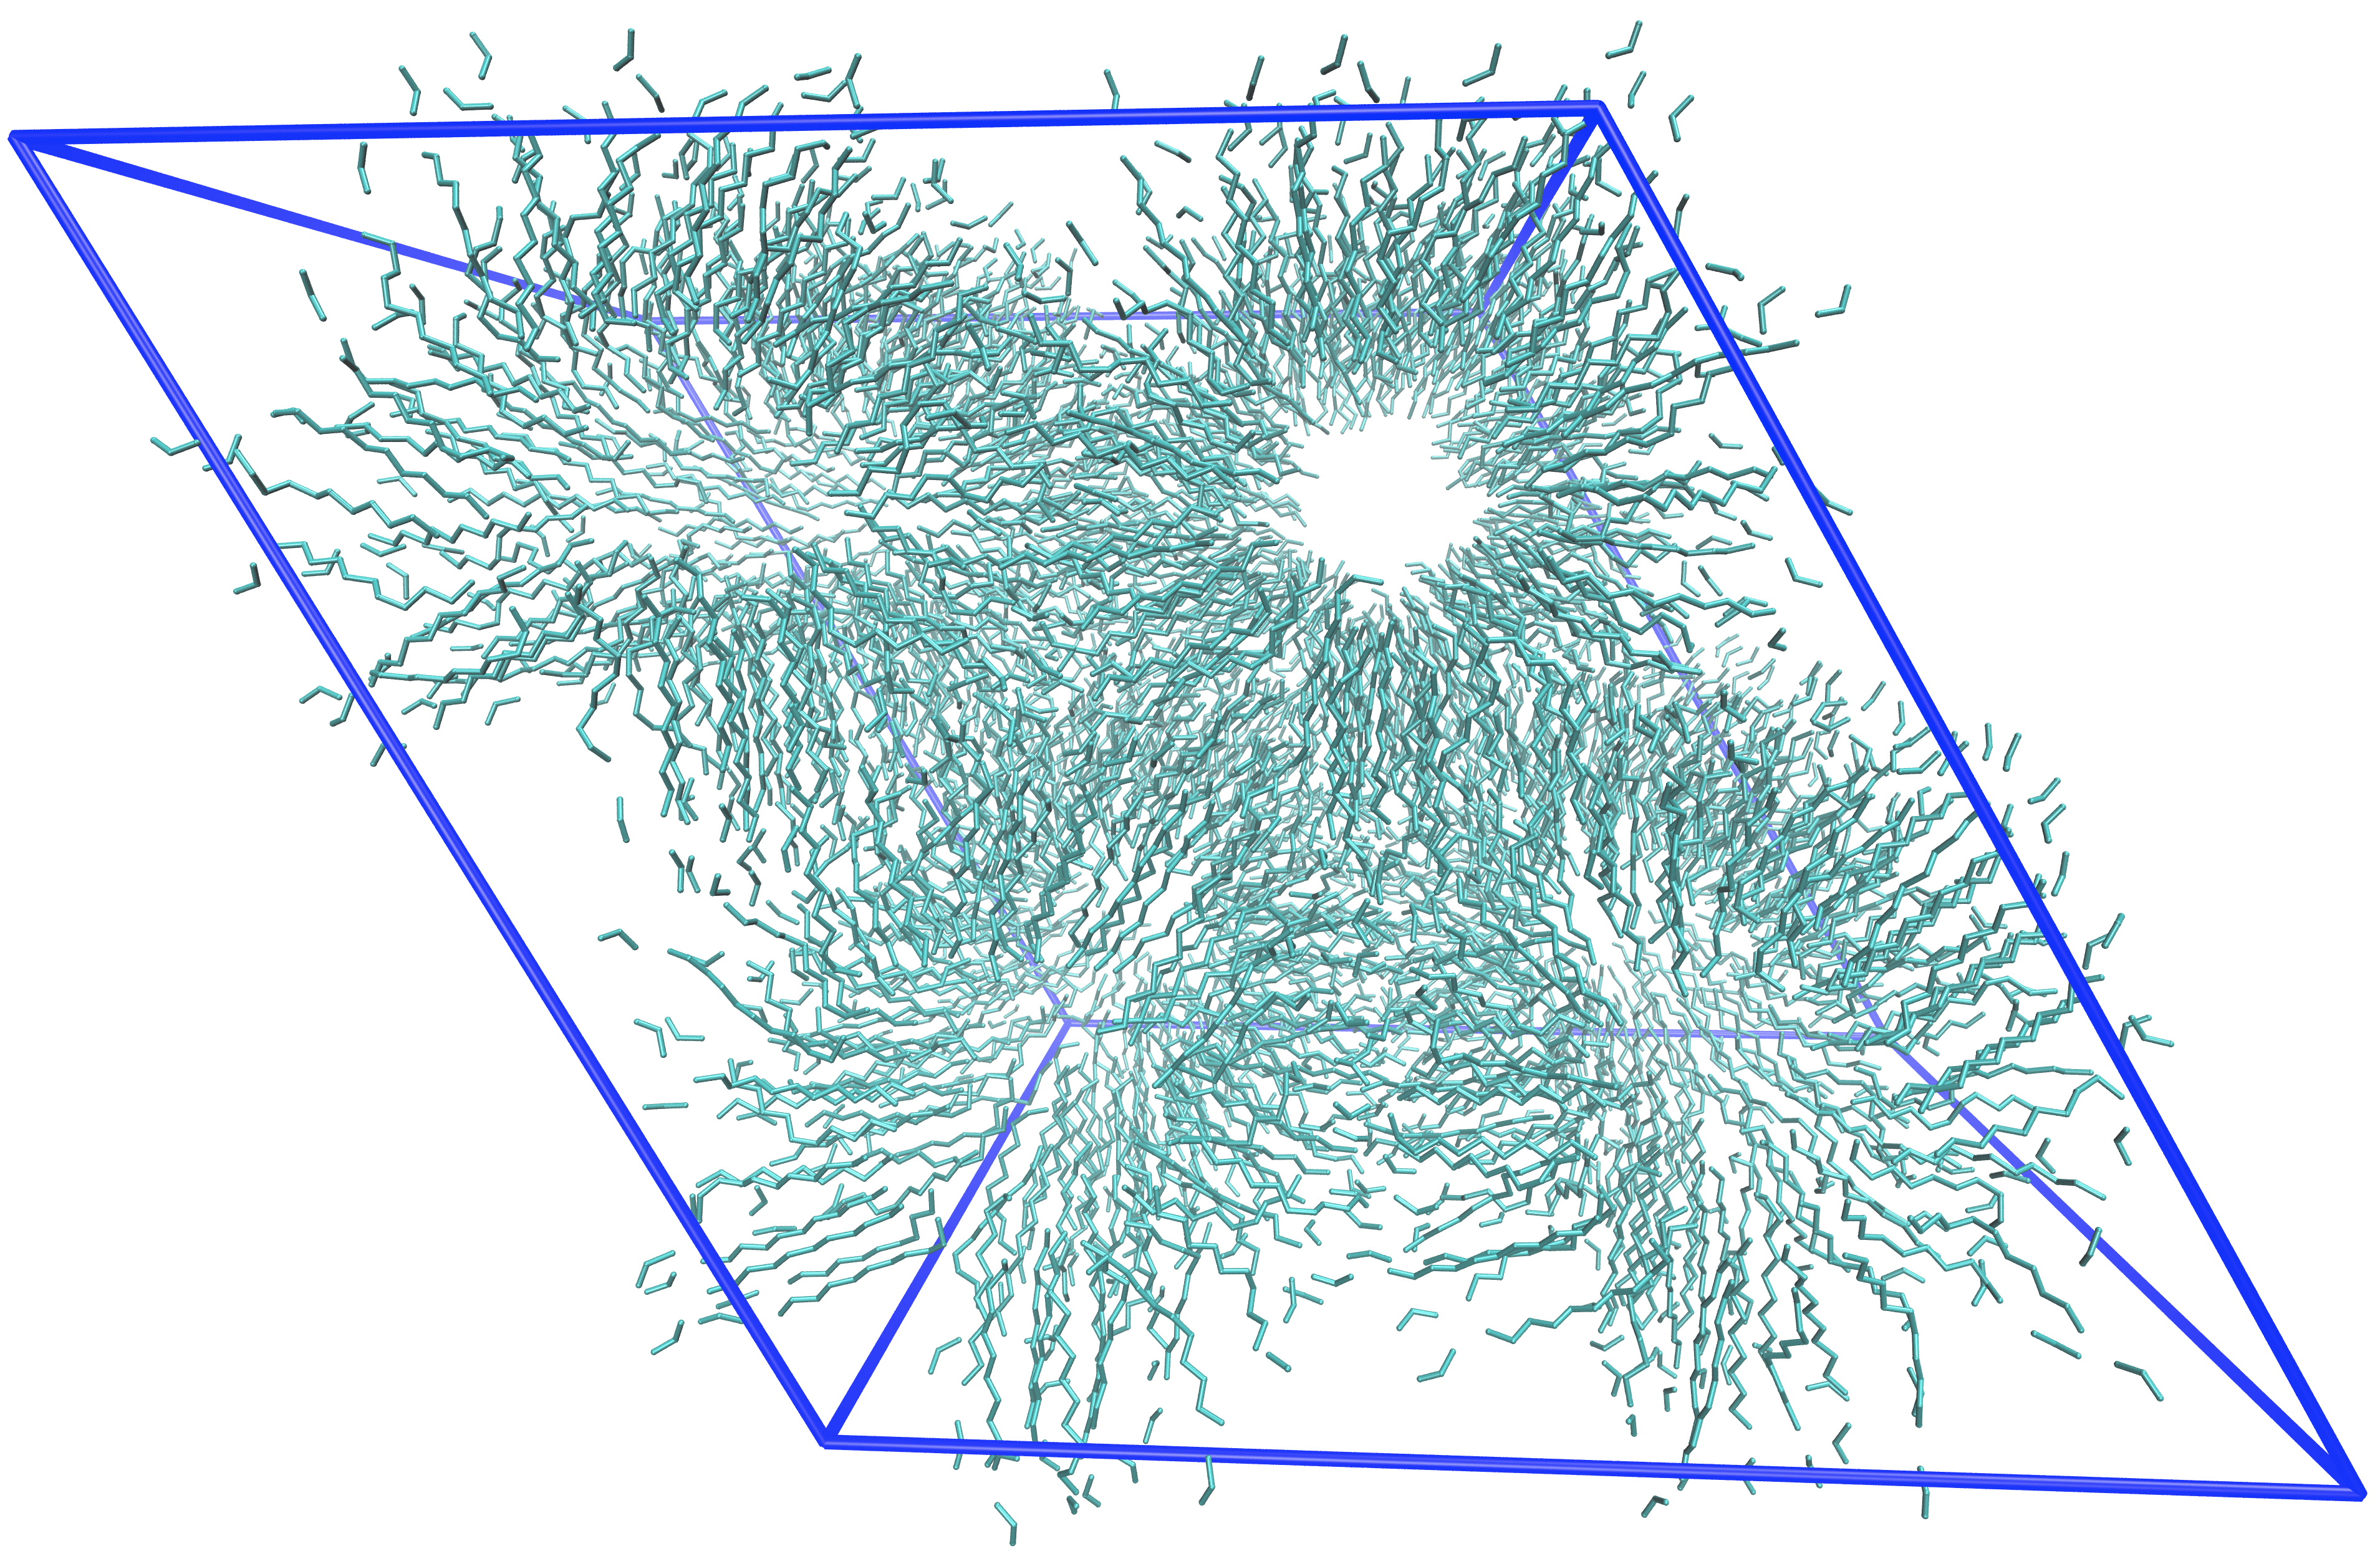
\includegraphics[width=\textwidth]{tails_topview.png}
		\caption{}\label{fig:tails_topview}
	\end{subfigure}
	\begin{subfigure}{0.45\textwidth}
		\centering
		\includegraphics[width=\textwidth]{tails_rzplot.png}
		\caption{}\label{fig:tails_rzplot}
	\end{subfigure}
	\begin{subfigure}{0.45\textwidth}
		\centering
		\includegraphics[width=\textwidth]{centroids_box.png}
		\caption{}\label{fig:centroids}
	\end{subfigure}
	\begin{subfigure}{0.45\textwidth}
		\centering
		\includegraphics[width=\textwidth]{angles_traj_layered.png}
		\caption{}\label{fig:angle_distribution}
	\end{subfigure}
	\caption{(a) The trajectory can be stripped of all atoms except carbon
	atoms in monomer tails. (b) Simulated diffraction of the tail-only trajectory
	still gives rise to R-spots. (c) Finding the center of mass and visualizing 
	their coordinates reveals the hexagonal-like packing of the tails. (d) The 
	distribution created by measuring the angle between each centroid (e.g. red 
	in (c)) and its neareset neighbors (e.g. green in (c)) with respect to the xy
	plane has distinct spikes near 30\degree, which is consistent with the location
	of R-spots}\label{fig:tail_packing}
\end{figure}

\subsection{Ionic conductivity calculation}

The model gives reasonable estimates of ionic conductivity for both phases.
Calculated values of ionic conductivity obtained using the Nernst Einstein
relation and Collective Diffusion model are compared in Table~\ref{table:conductivity}.
The two methods agree with each other within error, although the 
uncertainty obtained using the Collective Diffusion model is much higher.
Much longer simulations are needed to lower the uncertainty.
For this reason we will likely only use the Nernst Einstein relation
in future calculations of this type. Interestingly, Basin B 
has a higher ionic conductivity than Basin A. Conductivity is enhanced in
Basin B due to a higher sodium ion diffusivity. Transport of sodium is
likely facilitated by the homgeneity of Basin B. Sodium ions have less
sites to move to in Basin A. Currently there is no experimental
evidence of this trend, but it may be the subject of a future study. 
In both cases, our calculated values for Basin A are higher than the 
experimental values, as expected. Some of the discrepancy is likely a result
of using an imperfect forcefield. However, the real system, although mostly
aligned and straight, has a distribution of azimuthal angles, meaning 
that the pores have a degree of tortuosity which lowers the effective 
ionic conductivity of the bulk membrane. The ordering from isotropic to
mostly aligned mesophases showed an 85 fold increase in ionic conductivity.
We would expect additional gains in a perfect system.

\begin{table}
\centering
\begin{tabular}{ccc}
\toprule
\multicolumn{3}{c}{Calculated Ionic Conductivity \si{\siemens\per\meter}} \\
\hline
Method & Basin A & Basin B \\
\midrule
Nernst Einstein & \num{(1.23$\pm$0.01)e-4} & \num{(1.76$\pm$0.02)e-4} \\
Collective Diffusion & \num{(1.40$\pm$0.32)e-4} & \num{(4.6$\pm$2.4)e-4} \\
Experiment & \num{(1.33$\pm$ 0.10)e-5} & -- \\
\bottomrule
\end{tabular}
\caption{Calculated ionic conductivity using Nernst-Einsten and Collective Diffusion 
agree within error. Both methods give calculated values of ionic conductivity which
are an order of magnitude higher than experimental values~\label{table:conductivity}}.
\end{table}

\subsection{Implementation of the crosslinking algorithm}

We applied the crosslinking algorithm to an equilibrated structure in Basin B.
The procedure will be repeated with Basin A in the near future.
The resulting crosslinked structure has an even distribution of
crosslinks between monomer tails of the same monomer, monomers stacked on  % table of values here
top of each other and monomers in other pores, including across periodic
boundaries. The pore spacing shrinks by $\approx$ 1 \angstrom and stays 
constant under a range of simulation conditions. Figure~\ref{fig:xlink} compares
the pore behavior of a system that was a crosslinked and simulated for 10 ns to 
the pore behavior of the same system taken just before crosslinking and run for 10 ns.
Rather than plotting an average pore spacing, each pore-to-pore distance is plotted
separately. Visually, one can tell that the crosslinked pores are locked in place. 
The smaller pore spacing is also apparent by comparing the two plots. 
The simulations discussed previously have not been crosslinked. Moving forward,
the sandwiched system will be crosslinked in Basin A and used for
transport studies.

\begin{figure}
	\centering
	\begin{subfigure}{0.31\textwidth}
		\centering
		\includegraphics[width=\textwidth]{p2p_diagram.png}
		\caption{}\label{fig:p2p_diagram}
	\end{subfigure}
		\begin{subfigure}{0.31\textwidth}
		\centering
		\includegraphics[width=\textwidth]{no_xlink_p2p.png}
		\caption{}\label{fig:no_xlink_p2p}
	\end{subfigure}
		\begin{subfigure}{0.31\textwidth}
		\centering
		\includegraphics[width=\textwidth]{xlink_p2p.png}
		\caption{}\label{fig:xlink_p2p}
	\end{subfigure}
	\caption{(a) The legends of the plots in (b) and (c) refer to the numbers shown.
	Each numbered circle represents a pore. Distances are measured along each of the 
	lines shown in addition to the distance from pore 1 to pore 4. (b) The positions
	of individual pores fluctuate in an uncrosslinked system. (c) The positions of
	individual pores in the crosslinked system are stable relative to the uncrosslinked
	system}\label{fig:xlink}
\end{figure}
